% !Mode:: "TeX:UTF-8"
%%  本模板推荐以下方式编译:
%%     1. PDFLaTeX[推荐]
%%     2. xelatex [含中文推荐]
%%  注意:
%%  1. 文件默认的编码为 UTF-8 对于windows,请选用支持UTF-8编码的编辑器。
%%   2. 若是模板有什么问题,请及时与我们取得联系,Email:latexstudio@qq.com。
%%   3. 可以到  https://ask.latexstudio.net 提问
%%   4. 请安装 最新版本的 TeXLive 地址:
%%   http://mirrors.ctan.org/systems/texlive/Images/texlive.iso

\documentclass{apmcmthesis}
\usepackage{gbt7714}
\usepackage{url}
%\usepackage{cite}
\bibliographystyle{gbt7714-numerical}
%%%%%%%%%%%%填写相关信息%%%%%%%%%%%%%%%%%%%%%%%%%%
\tihao{A}                            %选题
\baominghao{2208185}                 %参赛编号
\begin{document}

\pagestyle{frontmatterstyle}
\begin{abstract}
	
Mould protection slag plays the role of heat preservation and oxidation prevention in continuous casting process. Therefore, the distribution of mould flux has been the focus of research in the metallurgical industry. In this paper, graphical processing methods and regression analysis are used to discuss the melting crystallization process of mould protection slag, which provides useful guidance for metallurgical industry to improve technology.

\textbf{For Task 1}, we design a high-precision text recognition model for the manually collected label graph of smelting key nodes to improve the efficiency of extracting image information. Firstly, the image is preprocessed, and then the \textbf{DenseNet model}is trained again based on \textbf{the CNOCR recognition} library. Finally, the accuracy of the model for the extraction of two groups of thermocouple temperature data is improved to \textbf{more than 98.8\%}. In addition, the reason for the large measurement deviation of the original image is inferred by mean analysis of the extracted temperature data.

\textbf{For task 2}, in order to comprehensively analyze the changing characteristics of image features over time, we extract the feature vectors of the images in Appendix 1 from five aspects: \textbf{gray feature, color feature,IBP feature, frequency feature and wavelet}. Then the within-group feature significance and between-group feature significance were analyzed using principal component analysis and box plots. The experimental results show that all the five features show strong significance. Based on this, the general Gaussian regression was used to fit the above mathematical model, and the melting and crystallization process of protection slag was analyzed and studied.

\textbf{For task 3}, in order to further analyze the relationship between the temporal characteristics and the melting crystallization thermodynamics of the protection slag, a \textbf{Gaussian process regression model} for the temperature and time of the \#1 and \#2 thermocouple was established based on the feature vectors of the existing keyframe images. Using a regression model as a prediction operator, we performed numerical simulations and fortunately found a polynomial relationship between temperature and melting period and die. Finally, polynomial regression was used to obtain the functional relationship between temperature and time changes and the melting and crystallization process of protective slag.


Finally, by searching the literature, the above models are reasonably evaluated and suggestions for the development of follow-up research are put forward.
\keywords{CNOCR\quad  DenseNet\quad Image processing \quad PCA\quad Gaussian process regression}
\end{abstract}


\newpage
%目录
\tableofcontents

\newpage
\pagestyle{mainmatterstyle}
\setcounter{page}{1}
\section{Introduction}

\subsection{Background}
		Mould flux plays the role of thermal insulation and preventing oxidation in the continuous casting process. \  The function of mould flux is mainly determined by the melting rate and crystallization rate of the flux under the temperature control curve.  \  Therefore, \  the distribution of mould flux has always been a key research direction in metallurgical industry.

		During smelting, \ the mould flux is continuously added to the liquid steel on the top of the container and accumulates in the form of powder on the surface of the liquid steel, \ which can prevent the crust of the liquid steel layer due to too fast cooling.
		
		After crystallization, \ it will eventually form three layers of slag film structure: glass layer, crystal layer and liquid slag layer. \ When the mould flux is completely fused, a layer of liquid slag will be formed on the surface of the molten steel. \ With the decrease of the longitudinal temperature of the mould liquid slag, \ the slag film attached to the wall of the copper plating mold was quenched and solidified to form a glass layer.\  At the end of smelting, \ the slag film appeared regional crystallization and formed a crystalline layer when the mould was forced to cool.
		
		As the phase transition of the mould flux is not easy to observe,with SHTT melting crystallization temperature tester, the researcher recorded the 562 crystallization behavior images of the mould flux from the $110^{th}$ second to $674^{th}$ second , see Attachment 1 and Figure 1-6, and the artificial identification information was recorded in the upper left corner of the key node image. In order to improve the recognition efficiency and facilitate scientific research, it is urgent to realize automatic feature extraction and model abstraction of images.
		
	\begin{figure}[htbp!]
	\begin{minipage}{0.33\linewidth}
		\centering
		\captionsetup{font={small}}
		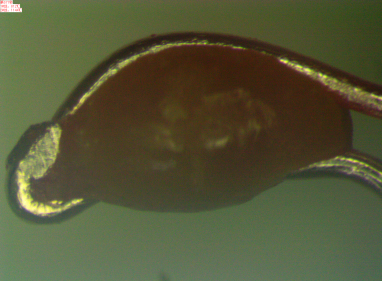
\includegraphics[height=3cm]{./figures/1-1.PNG}
		\caption{The sample}
		\label{fig:1}
	\end{minipage}
	\begin{minipage}{0.33\linewidth}
		\centering
		\captionsetup{font={small}}
		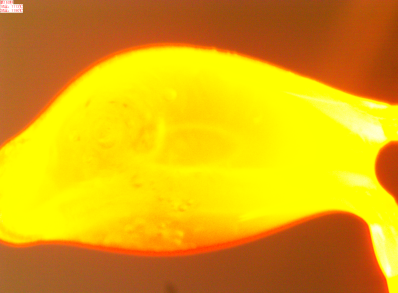
\includegraphics[height=3cm]{./figures/1-2.PNG}
		\caption{Begins to melt at 110s}
		\label{fig:2}
	\end{minipage}
	\begin{minipage}{0.33\linewidth}
	\centering
	\captionsetup{font={small}}
	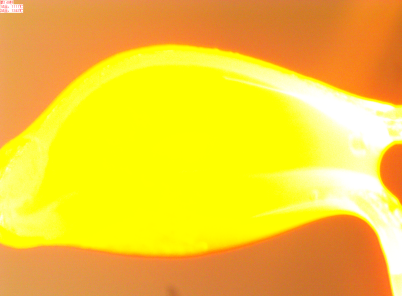
\includegraphics[height=3cm]{./figures/1-3.PNG}
	\caption{Completely melted at 141s}
	\label{fig:3}
\end{minipage}
\end{figure}
\begin{figure}[htbp!]
	\begin{minipage}{0.33\linewidth}
		\centering
		\captionsetup{font={small}}
		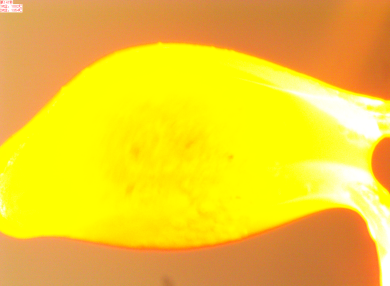
\includegraphics[height=3cm]{./figures/1-4.PNG}
		\caption{Sees steels melting at 149s}
		\label{fig:4}
	\end{minipage}
	\begin{minipage}{0.33\linewidth}
		\centering
		\captionsetup{font={small}}
		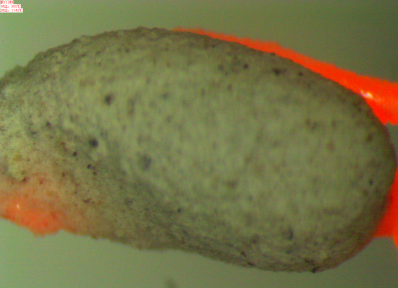
\includegraphics[height=3cm]{./figures/1-5.PNG}
		\caption{Crystallize begins at 150s}
		\label{fig:5}
	\end{minipage}
	\begin{minipage}{0.33\linewidth}
	\centering
	\captionsetup{font={small}}
	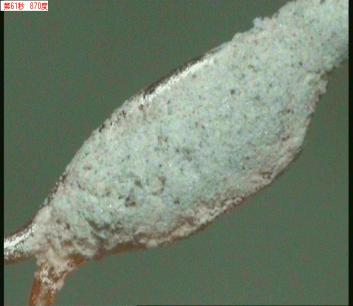
\includegraphics[height=3cm]{./figures/1-6.PNG}
	\caption{Crystallize ends at 671s}
	\label{fig:6}
\end{minipage}
\end{figure}
	
\subsection{Restatement of the Problem}
      	
\noindent\textbf{Task 1: } Please use Image Recognition to establish a mathematical model to realize the automatic extraction and data filling of  \# 1 \& \# 2 thermocouple temperature of key node image. By the way,a technical document is expected. \ In addition, make a temperatture-time curve diagram , point out and explain the test source of error of 1\# wire or 2 \# wire results.

\noindent\textbf{Task 2: } According to 6 node images in Figs 1, the dynamic differences between adjacent sequence images in the process of melting and crystallization are to quantify by digital image processing . Based on Time Series Analysis on different characteristics,establish the simulation model and discuss the melting crystallization process curve.
      	
\noindent\textbf{Task 3: } Please discuss relationship of function between the temperature and time evolution of the crystallization \& melting process. Then, discuss the kinetics of melting \& crystallization of mold fluxes with numerical simulation methods,  including temperature, melting rate and crystallization rate.

\subsection{Our Work}
	
	Based on the existing node image, we need to design a character recognition model to automatically collect the temperature data of the thermocouple and draw a curve to analyze the measurement error. Meanwhile, image feature extractor and time series model are also expected to be established. In addition, I should analyze the analytical relationship between temperature and time in the process and discuss kinetics of melting and crystallization.
	
\section{Problem analysis}

	\noindent\textbf{2. 1 Analysis of Task 1}
		
		After preliminary observation of Annex 1, in order to achieve accurate extraction of label information, it is necessary to preprocess the picture to improve the effective information density. There are many methods to realize text recognition through image processing technology, but it is necessary to select a model with high accuracy and strong and robust. After collecting the temperature data through the identification model, the program can be used to automate the filling of the form. Since the node image is acquired manually, the temperature error is inevitable due to the different measurement methods received.
		
	\noindent\textbf{2. 2 Analysis of Task 2}
	
    	The node image can reflect the time series change of the sample state characteristics with the melting time. We need to extract the effective pixels of the sample in the image and establish a time series model for analysis. We consider achieving pixel-level quantization and drawing curves by computer simulation, according to which dynamic changes can be visually reflected.

	\noindent\textbf{2. 3 Analysis of Task 3}
		
		There are different temperatures in different stages of ore melting and crystallization. Sufficient samples are given in the attachment. Based on the temperature recognition model of task 1 and the pixel change curve simulated by task 2, the functional relationship can be analyzed by feature extraction and dimension reduction and compression.
		
\section{Assumption}
	\begin{itemize}
	  \item All the indexes of water vapor and dust in the production environment meet the production requirements and will not have adverse effects on smelting.
	  
	  \item The temperature measurement of the two groups of thermocouples of the equipment is accurate and there is no instrument error. However, there are measurement errors due to manual observation.
	  
	  \item The quality of the image acquired by the instrument meets the basic requirements of image processing and the resolution of the camera is high enough.
	\end{itemize}
\section{Symbol Description}
	\begin{center}
	\small
	\captionsetup{font={small}}
	\tabcolsep=0.05cm
	\renewcommand\arraystretch{3}
	\begin{tabular}{ccc}
		\toprule
		\hline
		\makebox[0.2\textwidth][c]{Symbol}	& \makebox[0.35\textwidth][c]{Meaning} & \makebox[0.15\textwidth][c]{Unit}	 \\ \hline
	
		$T1_{i}$,$T2_{i}$& \#1 temperature   and \#2 temperature at the $i^{th}$second & \textcelsius \\ \hline
		$\mu $,Std   & First order color moment&  -\\ \hline
			$\eta,\lambda,\xi $   & First,second and -more order color moment,&  -\\ \hline
		$LBP$    &Linear Back Projection &  -\\ \hline
		$X,Y,C$	    & Input Set,Output Set, Kernel Function Matrix&  -\\ \hline
		$P,p$	    & Gaussian probability compensation function,Probability value&  -\\ \hline
		\bottomrule
\end{tabular}
\end{center}

\section{Model of Task 1 }

\subsection{Dataset pre-processing}
		
		For purpose on the improvement of the extraction accuracy of the key information of the node image, it is necessary to standardize the detection image to improve the enrichment of the effective information of the target.
		
		\noindent\textbf{5.1.1 Image cropping}
		
	 	Task 1 is to extract the temperature data of thermocouple \#1 and thermocouple  \#2 in the top-left corner of the dataset, so only the top-left region of the image contains valid data. If the original image is directly used for processing, due to the small area of the upper-left label in the image, direct recognition is not conducive to the convergence of the model and will produce large errors. If the proportion of the target image is too large, it will also increase the recognition error. Therefore, we consider the use of image processing techniques to crop the data map to the upper left $200\times100$ pixel range as the target label to make a new sample set,shown as following Figure7.
	 
		\begin{figure}
			\centering
			\captionsetup{font={small}}
			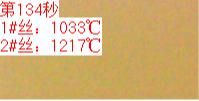
\includegraphics[height=2cm]{./figures/5-1.png}
			\caption{Slice of the image after preprocessing}
			\label{fig:8}
		\end{figure}
	
		\noindent\textbf{5.1.2 Target Limitation}
			
		Task 1 also requires to automatically fill in the table after extracting data. In the table in Attachment 2, the data are required to include: detection time, \#1 temperature, \#2 temperature, and the two target temperature variables are stipulated as $T1_{i}$,$T2_{i}$,denoting \#1 temperature   and \#2 temperature at the $i^{th}$second .
		
		In addition, according to the meaning of the question, the image of the attached data set is recorded from the $110^{th}$ second to the $674^{th}$ second. In order to facilitate the recording of the time, we have renamed the image file in batch and named it as "110", "111",... , "674", facilitating aspects of image management,operation and manual review.
		
		
\subsection{Model Building——CNOCR}
	
	   \noindent\textbf{5.1.1 Introduction to OCR }  
		
		Optical Character Recognition (OCR), it converts all kinds of printed text into image information through optical input methods such as scanning, and then extracts effective computer input information from the image by using character recognition technology.
		
		Using OCR technology can realize the extraction of the target text, text recognition is divided into Chinese, English and so on. In this case, the label map includes Chinese, numbers, and symbols. Finally, we will consider using the CNOCR library in Python to train the recognition model. CNOCR is an OCR toolkit that supports the recognition of Chinese, English and numbers in Python3. It supports the recognition of vertical characters and supports secondary development. We consider training the character recognition model of this problem on the basis of CNOCR.
		
		\noindent\textbf{5.1.2 DenseNet in CNOCR}  
		
		Convolutional Neural Network (CNN) is one of the most popular methods,and DenseNet is a dense connection based on CNN, where the preceding layers are connected to the following layers. Specifically, each layer accepts all the preceding layers as its additional input. In DenseNet, each layer is concatenated with all previous layers in the channel dimension (concat) and used as input to the next layer. For a L-layer network, DenseNet contains a total of $\frac{L(L+1)}{2}$ connections, and DenseNet directly concat feature maps from different layers, which can realize feature reuse and improve efficiency.
		
			
		\begin{figure}[htbp!]
		\centering
		\captionsetup{font={small}}
		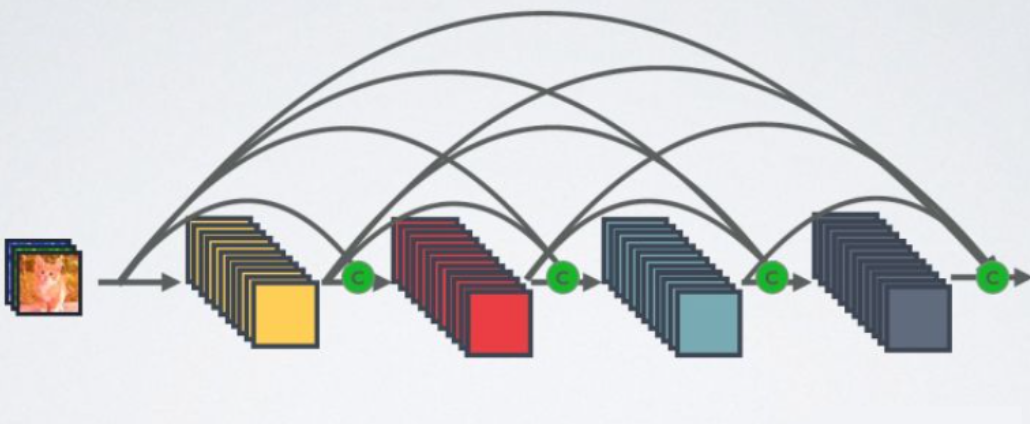
\includegraphics[height=5cm]{./figures/5-6.png}
		\caption{Dense connectivity mechanism for the DenseNet network}
		\label{fig:8}
		\end{figure}
	
	We adopt the CNOCR framework to implement DenseNet. CNOCR has built-in DenseNet and Densenet-Lite models. Here is a brief introduction to the training process:
	
\noindent\textbf{1)Input Layer}
		
		In DenseNet, all previous layers are concatenated as input:
		
		\begin{equation}
			\tag{5-2-1}
			  X_{k} = H_{k}([x_{0},x_{1},\cdots,x_{k-1}])
			\end{equation}
		
		The $H_{k}$ stands for non-liear transformation, which is a composition operation that may include a series of BN, ReLU, Pooling and Conv operations.


\noindent\textbf{2)Output Feature}

	\begin{figure}
		\centering
		\captionsetup{font={small}}
		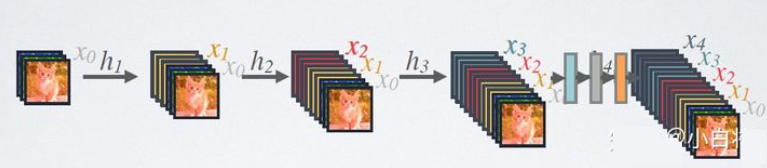
\includegraphics[height=3cm]{./figures/5-7.png}
		\caption{The forward process of DenseNet}
		\label{fig:8}
	\end{figure}
	
	Filled boxes are tensors allocated to memory, while translucent boxes are Pointers. Full arrows represent computations and dashed arrows represent memory Pointers. The efficient implementation stores the output of the join layer, batch normalization layer, and reread layer in a temporary storage buffer, while the original implementation allocates new memory.
		
	The Transition module connects two adjacent Denseblocks and reduces the feature map size by Pooling. Figure 9 shows the network structure of DenseNet, which contains a total of 4 Denseblocks connected by transitions.

	Features from input Layers are integrated and standardized by concat. After multiple convolutions, the input data is reduced to one dimension. The text pixel information on the picture is propagated forward for many times to finally compress the target features and extract the text.

\subsection{Model solving process}
	
	\noindent\textbf{5.3.1 CNOCR processing}
		
	We use the DenseNet model in CNOCR to train the set of images obtained by preprocessing. We divide the dataset into training set, test set and validation set. Since the model is relatively mature, we will use the first 100 groups of images for training to find a more suitable parameter configuration, and then use 50 groups of data for testing. After testing, the accurate recognition rate of the model can reach \textbf{98.5\%}.

	After that, we used the trained network to recognize all 564 groups of images, and used pandas to automatically write the obtained text data into the table in Annex 2, as shown in Table 1 below. Due to space reasons, only the first 16 groups of text recognition results are taken:
	
	
	
	% Please add the following required packages to your document preamble:
	% \usepackage{booktabs}
	\begin{table}[htbp!]
		\centering
		\small
		\caption{Thermocouple temperature identification results}
			\begin{minipage}{0.49\linewidth}
				\begin{tabular}{@{}cccc@{}}
				\toprule
				\textbf{NO} & \textbf{Time} & \textbf{1\# Temperature} & \textbf{2\# Temperature} \\ \midrule
				1           & 110           & 900                      & 1142                     \\
				2           & 111           & 904                      & 1146                     \\
				3           & 112           & 910                      & 1146                     \\
				4           & 113           & 914                      & 1144                     \\
				5           & 114           & 918                      & 1144                     \\
				6           & 115           & 923                      & 1146                     \\
				7           & 116           & 927                      & 1146                     \\
				8           & 117           & 932                      & 1146                     \\ \bottomrule
			\end{tabular}
		\end{minipage}
		\begin{minipage}{0.49\linewidth}
		\begin{tabular}{@{}cccc@{}}
			\toprule
			\textbf{NO} & \textbf{Time} & \textbf{1\# Temperature} & \textbf{2\# Temperature} \\ \midrule
			9           & 118           & 935                      & 1148                     \\
			10          & 119           & 938                      & 1146                     \\
			11          & 120           & 942                      & 1146                     \\
			12          & 121           & 947                      & 1153                     \\
			13          & 122           & 951                      & 1267                     \\
			14          & 123           & 953                      & 1418                     \\
			15          & 124           & 959                      & 1377                     \\
			16          & 125           & 965                      & 1218                     \\ \bottomrule
		\end{tabular}
		\end{minipage}
	\end{table}

	\noindent\textbf{5.3.2 Temperature change curve and anomaly analysis}
	
	Based on the temperature information obtained by the character recognition model, the temperature change curves of \#1 thermocouple and \#2 thermocouple with respect to time were drawn by MATLAB program, as shown in Figure 10:
	
	\begin{figure}
		\centering
		\captionsetup{font={small}}
		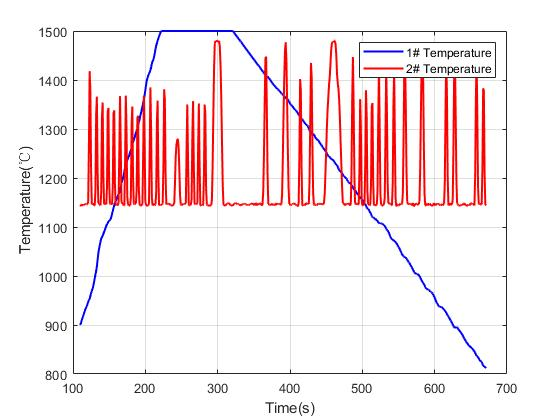
\includegraphics[height=6cm]{./figures/5-2.jpg}
		\caption{1\# wire temperature-2\# wire temperature-time diagram}
		\label{fig:8}
	\end{figure}
  
  	It can be seen from the image that the thermocouple \#1 shows a steady warming trend during the heating stage and a uniform decrease in temperature during the crystallization, but there is a constant temperature interval between the two states.
  	
  	Referring to the relevant literature and the manual of SHTT experiment instrument, we analyzed and inferred the possible reasons as follows: 
  	
  	1) After the melting reaches the melting point continue to absorb heat will not rise.
  	
  	2) SHTT experimental instrument has a thermal insulation function between the melting and crystallization stages of the sample.
  	
  	There is a certain correlation between the test data of the two groups of thermocouples. According to the requirements of the topic, we calculated the average temperature of the thermocouple at each time, and drew the average temperature curve of the thermocouple \#1 \& \#2 as shown in Figure:
\begin{figure}
	\centering
	\captionsetup{font={small}}
	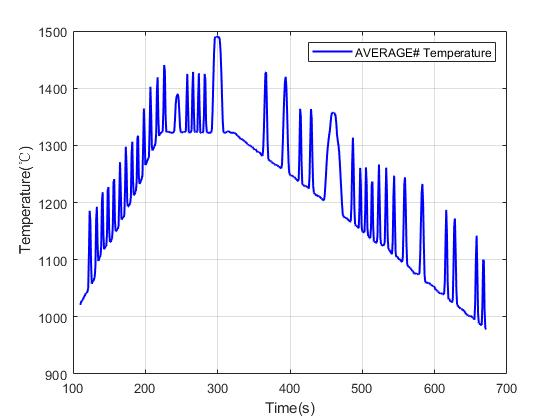
\includegraphics[height=6cm]{./figures/5-3.jpg}
	\caption{1\#wire average temperature-2\#wire average temperature-time diagram}
	\label{fig:9}
\end{figure}
	
	\subsection{Handbook of CNOCR Model}
		
		\noindent\textbf{Environment:}
		
		The temperature information text recognition model of task 1 is developed based on Python3, and depends on CNOCR library for secondary training. Before using this recognition software, you should ensure that the Python environment of version 3.7 or above is installed on the computer, and the third-party libraries referenced by this program are installed according to the following instructions:
		
	\noindent\textbf{Install Dependence:}
			
		\begin{tcode}
		pip install cnocr
		pip install pandas
		pip install re
		pip install Image
		\end{tcode}	
	If the installation speed is slow, you can specify the domestic installation source, such as using Douban source:
		\begin{tcode}
		pip install cnocr -i https://pypi.doubanio.com/simple
	\end{tcode}	
	
	\noindent\textbf{Warning:}
	
		If you have never installed PyTorch, OpenCV python packages on your computer, you may encounter problems with the initial installation, but they are generally common problems that can be solved by Baidu /Google.	
		
		
   	\noindent\textbf{Steps:}	
   	
   	\textbf{Step.1:}  Place the collected original picture in the path D disk path "D:\\Attachment 1".
   	
   	\textbf{Step.2:}  Place the table in Appendix 2 in the same directory as the python program task1.py.
   	
   	\textbf{Step.3:} Use Powershell or Pycharm and other IDE software to start the python program, pay attention to use "administrator mode" to ensure that the program has read and write the target file permissions.
   	
   	\textbf{Step.4:} Finally, the temperature information will be collected and written to the Attachment 2.xlsx file in the directory
\section{Model of Task 2}
	\subsection{Image Rough analysis}
		\noindent\textbf{6.1.1 Selection of extracted features}
		
		The sample feature map of ore is included in the question stem. In order to comprehensively reflect the change situation of each characteristic index of ore in the smelting and crystallization process, it is necessary to increase the coverage of the number of indicators as much as possible when designing characteristic indexes, so as to improve the comprehensivity of feature extraction.
		
		When selecting features, it can be cut from multiple dimensions, such as hue, color, pixel, etc., usually including the extraction of color features and texture features, and each sub-divided into a number of features can be used.
		
		\noindent\textbf{6.1.2 Ore smelting stage}
		
		Observing the image in the melting stage, we find that the color brightness of the image during melting is high, and the color concentration is dense, and the contrast is obvious. The corresponding image features can be extracted by pixel compression. At this time, the cosolvent is still in play, the image is bright, and the sample boundary is clear.
		
		\noindent\textbf{6.1.3 Ore crystallizing stage}

	In the crystallization stage of the image, we found that: with the advance of time, the sample temperature gradually decreased, and eventually the image would crystallizate into low-brightness objects, and the sample center approached to form the slag film first, and the coverage of the slag film would gradually increase the cooling rate. When the slag film layer was completely covered, the glass layer would be formed when the temperature continued to cool.
	
	\subsection{Model Building——5-domains feature extractor}
	\noindent\textbf{6.2.1 Grayscale feature Extractors}
	
		Co-occurrence gray matrix can reflect the comprehensive information of image gray level about adjacent interval, direction and amplitude. GLCM is generally determined by statistics of specific gray levels of the image and the state between pixels, and then seven statistics based on GLCM are calculated, including mean,sid angular second moment, contrast, correlation, dissimilarity, entropy, homogeneity and energy. The gray-level features of the image are explained:
		\begin{figure}[htbp!]
		\centering
		\captionsetup{font={small}}
		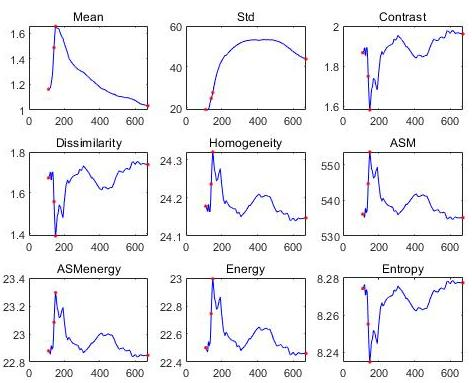
\includegraphics[height=5cm]{./figures/6-2-color.jpg}
		\caption{Curves of the 9 items of Grayscale features over time}
		\label{fig:9}
	\end{figure}
	
		Definition formula of 9 gray feature indexes is shown as below
			\begin{equation}
				\tag{6-2-1}
				\begin{split}
					Mean &= \frac{1}{i\cdot j}\sum_{i}\sum_{j}G(i,j) \\
					Std &= \sum_{i}\sum_{j}(i-Mean)^{2}\cdot G(i,j) \\
				   	ASM &= \sum_{i}\sum_{j}G(i,j)^{2} \\
					  Contrast &= \sum_{i}\sum_{j}(i-j)^{2}G(i,j) \\
						Correlation &= \sum_{i}\sum_{j}\frac{(i-\mu_{x})(j-\mu_{x})}{\sigma_{x}\sigma_{y}} \\
						Dissimilarity &= \sum_{i}\sum_{j}|i-j|^{k}G(i,j) \\
						Entropy &=-\sum_{i}\sum_{j}G(i-j)log(G(i,j)) \\
						Homogeneity &= \sum_{i}\sum_{j}\frac{G(i,j)}{1+|i-j|^{2}}\\
						Energy &= \sqrt{\sum_{i}\sum_{j}G(i,j)}
				\end{split}
			\end{equation}
		Where G(i, j) is the element value of the gray level co-occurrence matrix:
		\begin{equation}
			\tag{6-2-2}
			\begin{split}
				\mu_{x} &= \sum_{i}\sum_{j}i\cdot G(i,j) \\
					\mu_{y} &= \sum_{i}\sum_{j}j\cdot G(i,j) \\
						\sigma_{x} &= \sum_{i}\sum_{j}(i-\mu_{x})^{2}\cdot G(i,j) \\
			\sigma_{x} &= \sum_{i}\sum_{j}(i-\mu_{y})^{2}\cdot G(i,j) \\
			\end{split}
		\end{equation}
		
		
	

		\begin{figure}[htbp!]
			\centering
			\captionsetup{font={small}}
			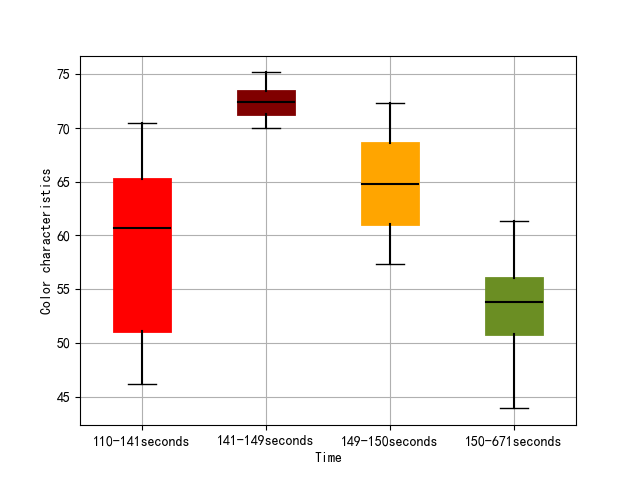
\includegraphics[height=6cm]{./figures/6-2-colorbx.png}
			\caption{Grayscale features of adjacent sequence images of melting crystallization process}
			\label{fig:9}
		\end{figure}
 \newpage
	
%	The color feature is described by the color feature of the image or image region, which has the integrity. Color feature extraction methods include color histogram, color set, and color moment. Taking color histogram extraction as an example, it is assumed that the integral of nonnegative function F (X) is 1:
%		\begin{equation}
%		\tag{6-2-1}
%		\int{F(X)d(X)}  = 1
%	\end{equation}
%
%If is not 1, the integral of F (X) is 1, so that equation (1) continues to be satisfied, then F (X) is the probability density function, and let the moment of X (order k) be:
%		\begin{equation}
%		\tag{6-2-2}
%		\phi_{k} = 	\int{r^{k}F(r)dr} \qquad k = 0, 1, 2,...
%	\end{equation}
%The central moment of order k is defined as:
%	\begin{equation}
%	\tag{6-2-3}
%	\psi_{k} = 	\int{(r - \phi_{1})^{k} F(r)dr} \qquad k = 0, 1, 2,...	
%\end{equation}
%
%	\begin{equation}
%	\tag{6-2-4}
%	\begin{split}
%	\phi{1}' = a_{0} \phi_{1}+b_{0} \\
%		\psi{k}' = a_{0}^{k} \psi_{k}
%		\end{split}
%\end{equation}
%
%The invariant is constructed from the central moment
%	\begin{equation}
%	\tag{6-2-5}
%	\begin{split}
%		f_{1} = \frac{\psi_{4}}{\psi_{2}^{2}} \quad
%		f_{1} = \frac{\psi_{6}}{\psi_{2}\psi_{4}} \quad
%		f_{1} =\frac{\psi_{8}}{\psi_{4}^{2}} 
%	\end{split}
%\end{equation}
%
%Second order center matrix
%
%
%	\begin{equation}
%	\tag{6-2-5}
%	\begin{split}
%	&\iint{F(x,y)dxdy} = 1\\
%	\phi_{k_{1},k_{2}} &= \iint{x^{k_{1}}y^{k_{2}}dxdy \qquad k_{1}, k_{2}\cdots}
%	\end{split}
%\end{equation}
%
%\begin{equation}
%	\tag{6-2-6}
%	\begin{split}
%	\Psi_{k_{1},k_{2}} = \iint{(x-\phi_{1,0}^{k_{1}})(y-\phi_{0,1}^{k_{2}})dxdy}\quad k_{1},k_{2} = 0,1,\cdots
%	\end{split}
%\end{equation}
%        \begin{equation}
%				\tag{6-2-7}
%				\begin{split}
%					\Psi_{1,0}'&= a_{1}\phi_{1,0}+b_{1}, \\
%					\Psi_{1,0}' &=a_{2}\phi_{0,1}+b_{2}, \\
%					\Psi_{k_{1},k_{2}}'&=a_{1}^{k_{1}}a_{2}^{k_{2}}\psi_{k_{1}k_{2}} \\
%				\end{split}
%		\end{equation}
%	


	\noindent\textbf{6.2.2 Color Feature Extractor}
	
	Color is one of the main features of an image. Color moment is a simple and effective color feature representation method, including first order moment, second order moment and third order moment. In this paper, the first, second and third order moments of three color components R, G and B are used to represent the color distribution of the molten crystallization process image of protection slag. The lower order moments can reflect the color distribution more comprehensively, and need not quantify the space. The three color moments are defined as follows.
	
    \begin{equation}
	\tag{6-2-3}
	\begin{split}
		\eta_{i}'&=\frac{1}{N}\sum_{j=1}^{N}P_{i,j} \\
		\lambda_{i}'&=\sqrt{\frac{1}{N}\sum_{j=1}^{N}(P_{i,j}-\eta _{i})^{2}} \\
		\xi_{i}' &= ^3\sqrt{\frac{1}{N}\sum_{j=1}^{N}(P_{i,j}-\eta_{i})^{2}} \\
	\end{split}
\end{equation}
	
	The first three order color moments of the three components of the image form a 9-dimensional vector, that is, nine color features are obtained.

%	\begin{figure}
%		\centering
%		\captionsetup{font={small}}
%		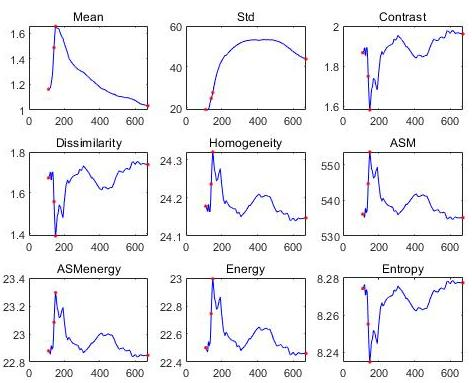
\includegraphics[height=6cm]{./figures/6-2-color.jpg}
%		\caption{Curves of the 9 items of color features over time}
%		\label{fig:9}
%	\end{figure}
	
	\begin{figure}
		\centering
		\captionsetup{font={small}}
		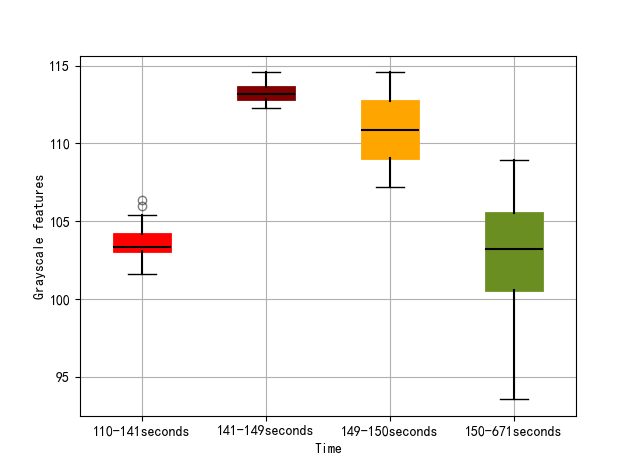
\includegraphics[height=6cm]{./figures/gray.png}
		\caption{Color features of adjacent sequence images of melting crystallization process}
		\label{fig:9}
	\end{figure}




\noindent\textbf{6.2.3 LBP Feature Extractor}

LBP refers to Local Binary Pattern, which is an operator used to describe the local features of images. LBP features have significant advantages such as gray invariance and rotation invariance.


The original LBP operator is defined in a 3×3 window and the center pixel of the window is used as the threshold.    Relative to the gray value of the 8 adjacent pixels, the position is marked as 1 if the value of the surrounding pixel is greater than the value of the middle pixel.    Otherwise, it will be marked as 0.

The principle of the traditional LBP model is as follows:


	\begin{equation}
			\tag{6-2-4}
			\begin{split}
				LBP(x_{c},y_{c}) &= \sum_{p = 1}^{8}s(I(p)-I(c))*2^{p} \\
				s(x) &= \begin{cases}	
					 1, x \geq 0 \\ 0, other
				  \end{cases}
			\end{split}
		\end{equation}
	
In order to improve the uniqueness of image features, this paper uses the improved feature model of LBP -- circular LBP. Ojala et al. improved the LBP operator by extending the 3×3 neighborhood to any neighborhood and replacing the square neighborhood with a circular neighborhood to improve the circular LBP. The principle of circular LBP is basically consistent with the traditional LBP, and the sampling points P and the radius R of the sampling circle field are introduced.


	\begin{equation}
	\tag{6-2-5}
		\begin{split}	
		&	LBP_{P,R}(x_{c},y_{c}) = \sum_{p = 1}^{P}s(I(p)-I(c))*2^{p} \\
		 &\begin{cases}
			x_{p} &= x_{c}+R\cdot cos(\frac{2\pi p}{P}) \\
				y_{p} &= y_{c}-R\cdot sin(\frac{2\pi p}{P}) 
			\end{cases}	\\
			&s(x) = \begin{cases}
			1, x \geq 0 \\ 0, other
		\end{cases}
	\end{split}
\end{equation}
According to the basic principle of LBP, we extract the original LBP features, rotation invariant LBP features, equivalent pattern LBP features and rotation invariant equivalent pattern LBP features of the image region, and draw the feature time series curve, as shown in the figure:


\begin{figure}
	\centering
	\captionsetup{font={small}}
	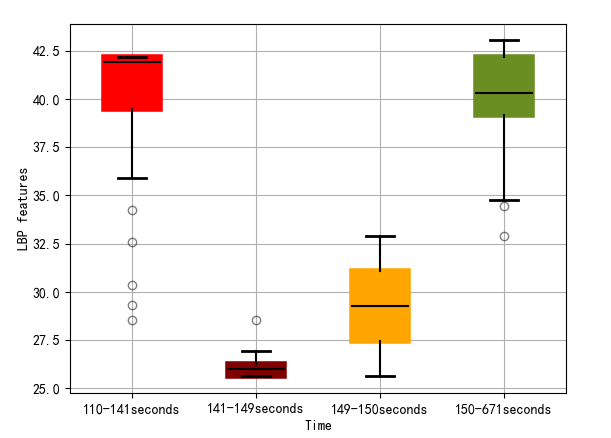
\includegraphics[height=6cm]{./figures/6-2-lbpxs.png}
	\caption{LBP features of adjacent sequence images of melting crystallization process}
	\label{fig:9}
\end{figure}


\begin{figure}
	\centering
	\captionsetup{font={small}}
	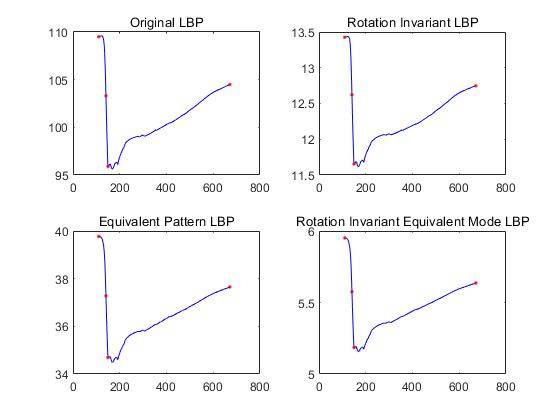
\includegraphics[height=6cm]{./figures/6-2-lbp.jpg}
	\caption{4 kinds of LBP feature time series curves}
	\label{fig:9}
\end{figure}

\noindent\textbf{6.2.4 Frequency Feature Extractor}	

We extracted the spectral frequency features of image pixels using fast Fourier transform (FFT), which is a discrete Fourier transform algorithm that is done in time of$O(n\log{n})$

To expand the target expression, we apply a polynomial transformation to obtain:
\begin{equation}
	\tag{6-2-6}
	\begin{split}	
		f(x)& = (a_{0}+a_{2}x^{2}+\cdots+a_{n-2}^{n-2})+(a_{1}^{1}+a_{3}^{3}+\cdots+a_{n-1}^{n-1}) \\
	Then: f(x)_{1} & = a_{0}+a_{2}x^{2}+\cdots+a_{n-2}x^{\frac{n}{2}-1} \\
	f(x)_{2} & =x(a_{1}+a_{3}x+\cdots+a_{n-1}x^{\frac{n}{2}-1})
	\end{split}
\end{equation}

With $x = \omega_{n}^{k}$ and $x = \omega_{n}^{k+\frac{n}{2}}$ relatively,then we get:
\begin{equation}
	\tag{6-2-7}
	\begin{split}	
		f( \omega_{n}^{k}) = f(\omega_{\frac{n}{2}}^{k})_{1}+\omega_{n}^{k}f(\omega_{\frac{n}{2}}^{k})_{2} \\
		f( \omega_{n}^{k+\frac{n}{2}}) =
	f(\omega_{\frac{n}{2}}^{k})_{1}-\omega_{n}^{k}f(\omega_{\frac{n}{2}}^{k})_{2} \\
	\end{split}
\end{equation}

Finally, we can convert to the transform target of FFT as below:
\begin{equation}
	\tag{6-2-8}
	fun = fsolve ( f(\omega_{1}^{k})+f(\omega_{2}^{k})  = 1)
\end{equation}
	\begin{figure}[htbp!]
	\centering
	\captionsetup{font={small}}
	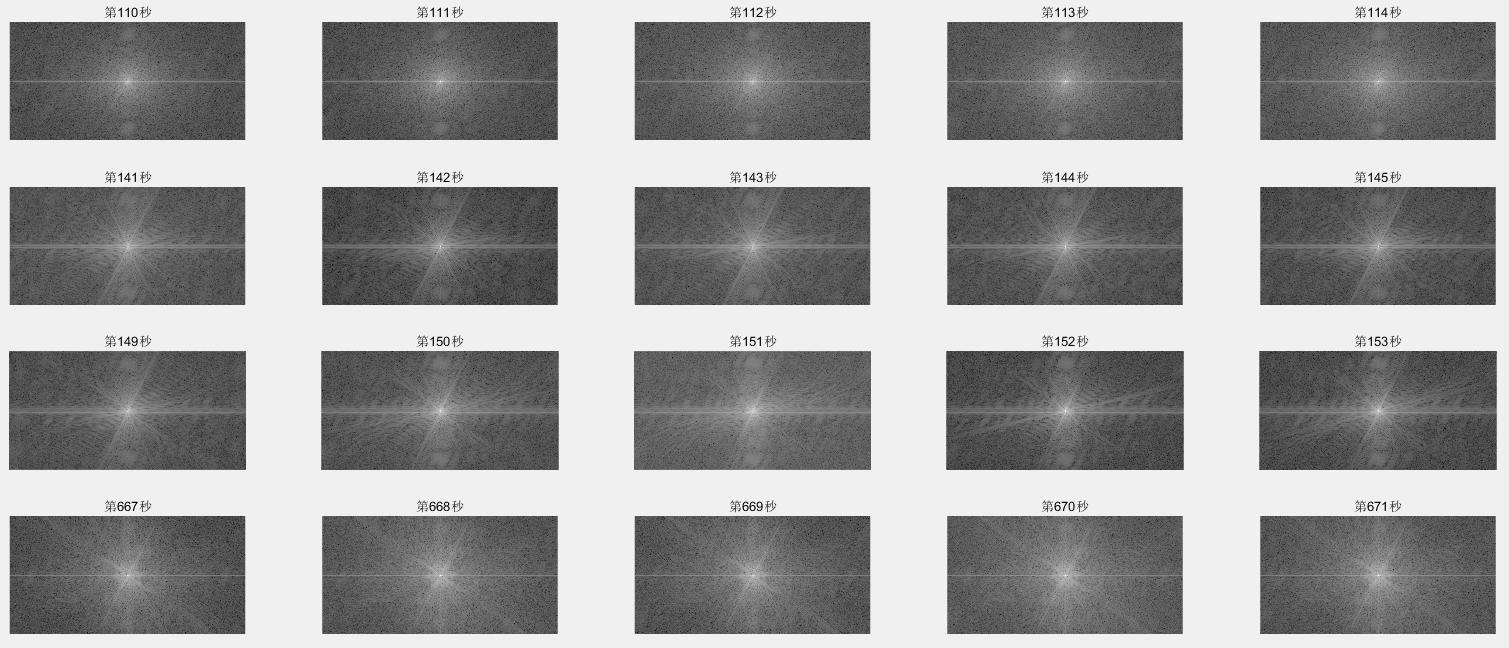
\includegraphics[height=6cm]{./figures/6-2-fre.png}
	\caption{Image spectral frequency feature map}
	\label{fig:9}
\end{figure}	

We selected 20 representative samples from the sample, and used fast Fourier transform to extract the frequency characteristics of the samples respectively:


\noindent\textbf{6.2.5 Wavelet  Feature Extractor}	

\noindent\textbf{(1)Dobbercy Wavelet transform decomposition}

The Coiflet wavelet is a discrete wavelet designed by Ingrid Daubechies. It can simultaneously have high vanishing momentum and its waveform is nearly symmetric, which is often used in digital signal processing. For image digital signal processing, it has strong extraction ability.

In order to improve the efficiency of the model, the use of discretization processing algorithm can greatly reduce the space complexity, and dyadic wavelet is commonly used to deconstruct two-dimensional image information:

2-Dimensional continuous wavelet transform:
\begin{equation}
	\tag{6-2-9}
	W_{f}(a,b_{x},b_{y}) = \int^{\infty}_{-\infty}\int^{\infty}_{-\infty}f(x,y)\Psi_{a_{x}b_{x}b_{y}}(x,y) = dxdy
\end{equation}
Inverse 2-Dimensional continuous wavelet transform
\begin{equation}
	\tag{6-2-10}
	f(x,y) = \frac{1}{C_\Psi}\int^{\infty}_{0}\int^{\infty}_{-\infty}\int^{0}_{-\infty}W_{f}(a,b_{x},b_{y})\Psi_{a_{x}b_{x}b_{y}}(x,y)db_{x} db_{y}\frac{da}{a^{3s}}
\end{equation}	
\begin{figure}[htbp!]
	\centering
	\captionsetup{font={small}}
	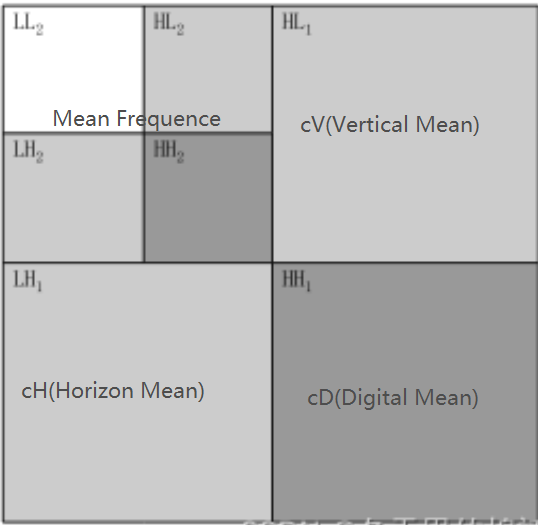
\includegraphics[height=4cm]{./figures/6-2-10.png}
	\caption{Component structure diagram of the Dobbercy wavelet decomposition}
	\label{fig:9}
\end{figure}
Two-dimensional discrete wavelet transform is the extension of one-dimensional discrete wavelet transform, which decomposes the signal in different scales, so as to obtain the myopic value and detail value of the original signal. Since the signal is two-dimensional, the decomposition is also two-dimensional; The results of the decomposition are: approximate components; Horizontal detail component; Vertical detail component; Diagonal detail component, in this paper, the image information is considered as the low-frequency input excitation as below:

1) Mean low frequency(cA)

2) Horizontal high frequency mean(cH)

3) Vertical high frequency mean(cV)

4) Diagonal high-frequency mean(cD)


		Using the Dobbercy wavelet, we extracted wavelet features for the detection image in problem 1, as shown in the figure is the wavelet feature curve during melting and crystallization.\newpage
\begin{figure}[htbp!]
	\begin{minipage}{0.49\linewidth}
		\centering
	\captionsetup{font={small}}
	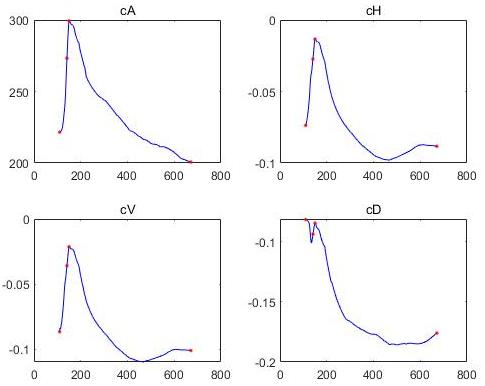
\includegraphics[height=4.5cm]{./figures/6-2-fe.jpg}
	\caption{Graph of wavelet characteristic during melting and crystallization}
	\end{minipage}
	\begin{minipage}{0.49\linewidth}
		\centering
		\captionsetup{font={small}}
		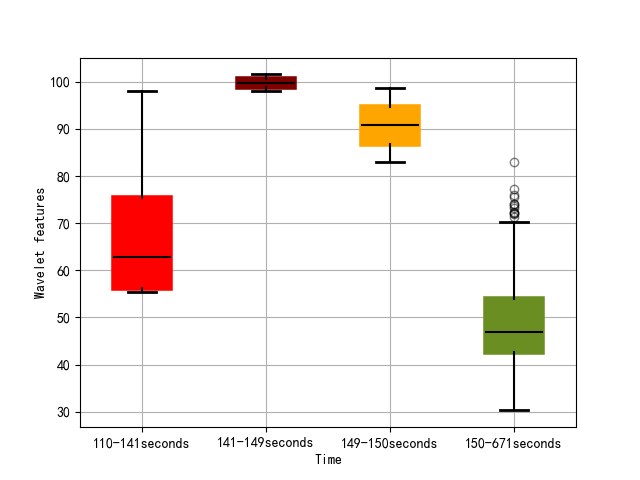
\includegraphics[height=4.5cm]{./figures/6-3-wave.png}
		\caption{Wavelet features of adjacent sequence images of melting crystallization process}
		\label{fig:9}
	\end{minipage}	
\end{figure}

	\subsection{Model solving process}
	
		Based on the above research model,  we successively extract five main types of image features as feature indicators in the smelting process. Due to the  large number of selected indicators,  it is necessary to screen the quality of indicators. We assume that the principal component analysis (PCA) is calculated  between adjacent sequence images in the melting and crystallization process of protective slag by using the five groups  of features extracted in time series:
		
		\begin{figure}[htbp!]
			\centering
			\captionsetup{font={small}}
			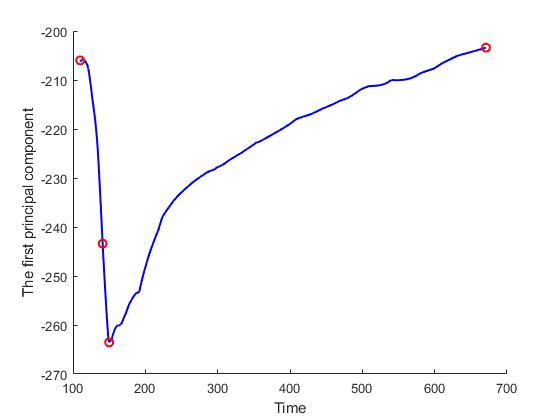
\includegraphics[height=5cm]{./figures/6-3-2.jpg}
			\caption{PCA feature quantity dimensionality reduction curve}
			\label{fig:9}
		\end{figure}
	
	

After the verification of principal component analysis, the extracted image features in the five fields have strong relationships with the smelting and crystallization process of ore samples. We fit the model by using the Gaussian process linear model with five groups of feature data, and the model parameters are as shown in Table 2:
	\begin{equation}
		\tag{6-3-1}
		\begin{split}
			f(x) = a_{1}e^{\frac{-(x-b_{1})}{c_{1}}^{2}}+a^{2}e^{\frac{-(x-b_{2})}{c_{2}}^{2}}
			\end{split}
	\end{equation}

	\begin{table}[htbp!]
		\centering
	\caption{Generic Gaussian model fitting parameters}
	\begin{tabular}{llll}
		\hline
		\textbf{Parameter} & \textbf{Min} & \textbf{Average} & \textbf{Max} \\ \hline
		\textit{$a_{1}$}   & 0.92         & 1.16             & 1.40         \\
		\textit{$b_{1}$}   & 723.50       & 810.90           & 898.30       \\
		\textit{$c_{1}$}   & 97.56        & 304.20           & 510.70       \\
		\textit{$a_{2}$}   & -0.19        & 0.20             & 0.60         \\
		\textit{$b_{2}$}   & 316.10       & 429.20           & 542.40       \\
		\textit{$c_{2}$}   & 151.90       & 213.10           & 274.40       \\ \hline
	\end{tabular}
\end{table}
According to the results of the model fitting, we plotted the melting and crystallization process curves of the protective slag in the melting and crystalline states:
	\begin{figure}[htbp!]
		\centering
		\captionsetup{font={small}}
		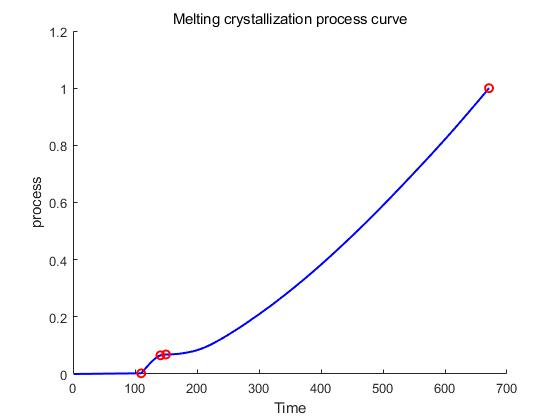
\includegraphics[height=5cm]{./figures/6-3-3.jpg}
		\caption{Melting and crystallization process curves}
		\label{fig:9}
	\end{figure}
	
	The melting and crystallization process curves of the protection slag in, in the melting stage:, the dynamic differences between adjacent sequence images do not change significantly, and the image characteristics of key nodes are similar, which are all highlighted. In the crystallization stage: Since the sample in the figure is rapidly cooled and crystallized, the characteristics of the crystallization stage change rapidly, and the change rate gradually slows down.
	
	
\section{Model of Task 3}
	\subsection{Rough analysis of relationship between temperature and time}
Based on the above extraction model of melting crystallization image features and the temperature data in Annex 2, we begin to analyze the temperature timing relationship.

The data in Annex 2 are extracted from the image set in Annex 1, which is limited to the accuracy of OCR. Within the allowable range of error, the regression method can be used to analyze the relationship between time and temperature.



We project the data extracted from task 1 into a three-bit space with time as the axis, and obtain the surface of the temperature of the two couples with respect to time, as shown in Figure 22:
	
			
	\begin{figure}[htbp!]
		\centering
		\captionsetup{font={small}}
		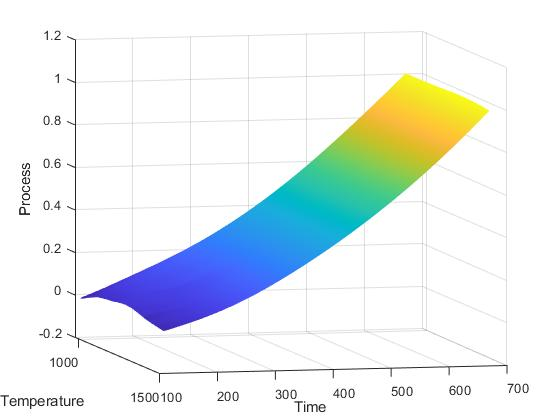
\includegraphics[height=4cm]{./figures/7-1.jpg}
		\caption{The surface of the thermocouple temperature with respect to time}
	\end{figure}


From the figure, it can be found that the surface is smooth without singularities and has strong linear correlation.Since there is a linear relationship between the variables, we consider analyzing the expression of the temperature using a polynomial regression model-Gaussian process regression is the typical polynomial regression model.
\subsection{Model Building——Gaussian process Regression}
	 \noindent\textbf{7.2.1 Gaussian process}
	In statistics, a Gaussian process refers to a probabilistic model in which observations occur in a continuous domain (Figure 23).  In a Gaussian process, a finite set of any random variables is required to satisfy a normal distribution, and continuous points in the input space are correlated with normally distributed random variables.  Gaussian process is commonly used in machine learning to measure the similarity of kernel function in sample space.  Based on a large amount of training data, Gaussian process can be used to predict points distributed at the edge of probability space.  The Gaussian process model is highly portable and suitable for regression prediction of nonlinear models.
	
		\begin{figure}[htbp!]
		\centering
		\captionsetup{font={small}}
		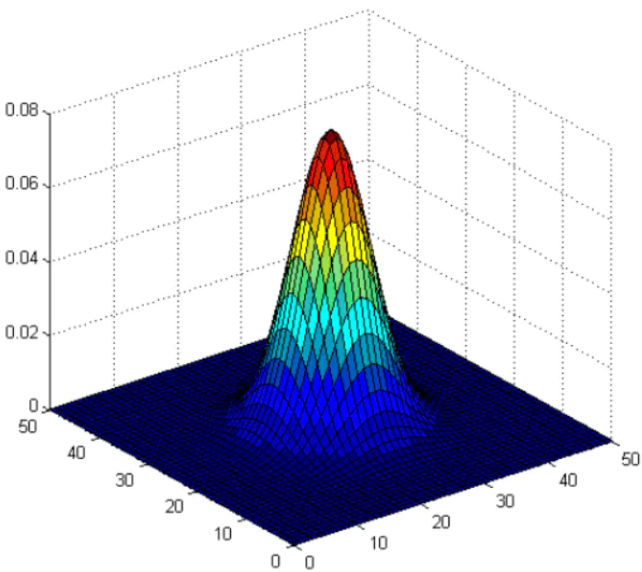
\includegraphics[height=4cm]{./figures/7-4.png}
		\caption{The surface of 2-dimensional Gaussian surface distribution
		}
	\end{figure}	
	
	\noindent\textbf{7.2.2 Principle of multivariate Gaussian distribution}
	
	Multivariate Gaussian distribution extends Gaussian distribution from one-dimensional variable to high latitude space, which makes Gaussian process regression model have stronger applicability. Multivariate Gaussian distributions in Gaussian probability compensation functions are derived as Equation 7-2-1 below:
	
	\begin{equation}
		\tag{7-2-1}
		\begin{split}
			P(x_{1},x_{2}\cdots,x_{n})& =\prod_{i=1}^{n}p(x_{i}) \\ &=\frac{1}{\prod_{j=1}^{n}\sigma_{j}\sqrt(2\pi^{\pi})}exp(-\frac{1}{2}\sum_{i=1}^{n}\frac{(x_{i}-\bar{x}_{i})^2}{2\sigma^2_{i}})
		\end{split}
	\end{equation}
	
	\noindent\textbf{7.2.3 Gaussian process regression Model}	
	
	\noindent\textbf{Step 1. }Determine the sampling point:
	\begin{equation}
		\tag{7-2-2}
		\begin{split}
			&X =\left[x_{1},x_{2},\cdots,x_{n}\right]	\\
			&Y=\left[y_{1},y_{2},\cdots,y_{n}\right]	\\
			&X\sim N(\bar{x}(t),C(t,t'))
		\end{split}
	\end{equation}
	\noindent\textbf{Step 2. }Identify the sample centers:
	
	In this model, in order to facilitate model derivation, the mean value $\bar{x_{i}}$is taken here so that the Gaussian distribution center is located at the origin
	
	\noindent\textbf{Step 3. }Squared Exponential Kernel function of Gaussian regression:
	
	\begin{equation}
		\tag{7-2-3}
		c(x,x'|\theta)=\sigma^{2}_{f}e^{\frac{-(x_{i}-x_{j})^{T}(x_{i}-x_{j})}{2\sigma_{l}^{2}}}
	\end{equation}

	\begin{equation}
		\tag{7-2-4}
		C(x,x')=\begin{bmatrix}
			c(x_{1},x'_{1}) &	c(x_{1},x'_{2})&\cdots&	c(x_{1},x'_{n}) \\
			c(x_{2},x'_{1}) & 	c(x_{2},x'_{2})	&\cdots&	c(x_{2},x'_{n})\\
			\vdots & \vdots & \ddots &\vdots \\
			c(x_{n},x'_{1})& 	c(x_{n},x'_{2})& 	\cdots&	c(x_{n},x'_{n})	
		\end{bmatrix}
	\end{equation}
	
	After debugging the model, the optimal parameters of Gaussian kernel function are as follows.
	
\qquad	\textbf{ $\sigma_{f} = 0.245369$ \qquad $\sigma_{l} = 0.013485$}
	 
	\noindent\textbf{Step 4. }Calculate the posterior probabilities:
	
	According to Bayes theorem, based on the data set of observations (X, Y), the posterior probability distribution of the Gaussian process can be calculated as follows:
	
	\begin{equation}
		\tag{7-2-5} 
		p(f\mid X,Y) \propto p(Y\mid X,f)p(f)
	\end{equation}
	\noindent\textbf{Step 5. }Regression fitting was performed:
	
	Based on the posterior probability distribution, time series samples in the data set can be collected and the selected feature indicators can be analyzed in turn:
	\begin{equation}
		\tag{7-2-6}
	   \begin{bmatrix} 
			y 	\\
			y^{*}
			\end{bmatrix} 
			\sim N\left(0,\begin{bmatrix} 
			C & C^{T}_{*} \\
			C_{*} & C_{**}
		\end{bmatrix} 
		\right)
	\end{equation}
	The matrix representation of covariance matrix, $C ^ {T} _ {*} = C_ {*} $,is predicted data collection observation covariance matrix between the data sets, $C_ {*} $said prediction covariance matrix of the data set; The resulting predicted values satisfy the following probability constraints:
	\begin{equation}
		\tag{7-2-7}
		p(y^{*}\mid x^{*},X,Y) = \int p(y^{*}\mid f^{*})p(f^{*}\mid x^{*},X,Y)df^{*}
	\end{equation}
	\subsection{Model solving process}
	
	\noindent\textbf{7.3.1 Gaussian regression predicts thermocouple temperature}
	
	According to the multivariate Gaussian process regression model established above, we regressed the \# 1 and \# 2 thermocouple temperatures extracted in Annex 2 on the image time respectively, so as to predict the corresponding thermocouple temperature at a certain time.
	
	\noindent\textbf{7.3.2 Numerical simulation and fitting}
		
		
%	\begin{equation}
%		\tag{7-3-1}
%		f(x) =  a_{1}\cdot e^{-(\frac{x-b_{1}}{c_{1}})^{2}} + a_{2}\cdot e^{-(\frac{x-b_{2}}{c_{2}})^{2}}
%	\end{equation}

	We used Gaussian process regression as the generator of the numerical simulation, and plotted the scatter plot using multiple sets of time prediction thermocouple plots. By observing the scatter plot of melting and crystallization phases, we found that the scatter plot of temperature change rate in melting phase showed a quadratic function distribution, and the scatter plot of temperature change rate in crystallization phase showed a first-order function distribution.
	
	\begin{figure}[htbp!]
		\centering
		\captionsetup{font={small}}
		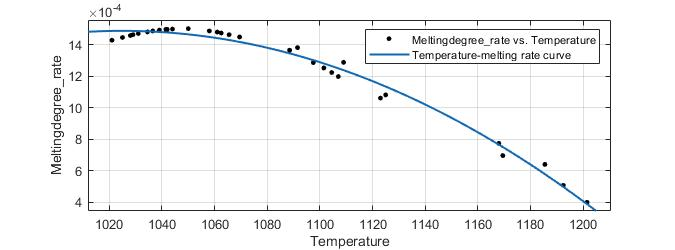
\includegraphics[height=5cm]{./figures/7-2.jpg}
		\caption{Temperature-melting rate curve}
	\end{figure}
	
	
	After predicting the temperature rate scatter through computer simulation, we used a quadratic linear regression model to regressively fit the temperature change rate during melting, and obtained the thermodynamic relationship curve of the melting stage:
	
	\begin{equation}
		\tag{7-3-1}
		f(x) =  p_{1}x^{2}+p_{2}x+p_{3}
	\end{equation}
	% Please add the following required packages to your document preamble:
	% \usepackage{booktabs}
	\begin{table}[htbp!]
			\caption{Model parameters of temperature and time during melting}
		\centering
		\begin{tabular}{@{}llll@{}}
			\toprule
			\textbf{Parameter} & \textbf{Min} & \textbf{Average} & \textbf{Max} \\ \midrule
			$p_{1}$            & -4.08E-08    & -3.53E-08        & -2.97E-08    \\
			$p_{2}$            & 6.01E-05     & 7.23E-05         & 8.46E-05     \\
			$p_{2}$            & -0.04233     & -0.03557         & -0.02881     \\ \bottomrule
		\end{tabular}
	\end{table}
\begin{figure}[htbp!]
	\centering
	\captionsetup{font={small}}
	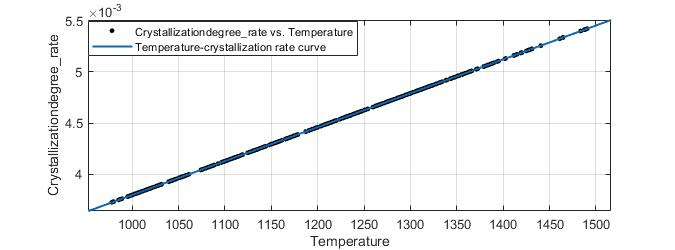
\includegraphics[height=5cm]{./figures/7-3.jpg}
	\caption{Temperature-time quadratic regression curve of the melting process}
\end{figure}
	
Similarly, we used computer simulation to predict the thermodynamic parameters of the mold for regression, and used a linear fitting model to regression the thermodynamic relationship curve of the crystallization stage. The relationship between temperature, melting rate and crystallization rate can be shown in the curve.

\begin{equation}
	\tag{7-3-2}
	f(x) =  p_{1}x+p_{2}
\end{equation}

% Please add the following required packages to your document preamble:
% \usepackage{booktabs}
\begin{table}[htbp!]
	\caption{Model parameters of temperature and time during crystallization}
	\centering
	\begin{tabular}{@{}llll@{}}
		\toprule
		\textbf{Parameter} & \textbf{Min} & \textbf{Average} & \textbf{Max} \\ \midrule
		$p_{1}$            & 3.31E-06     & 3.31E-06         & 3.31E-06     \\
		$p_{2}$            & 4.84E-04     & 4.84E-04         & 4.84E-04     \\ \bottomrule
	\end{tabular}
\end{table}

	

\section{Strengths and Weakness}

\noindent\textbf{8.1 Evaluation of Model 1}

\noindent\textbf{8.1.1 Strengths of CNOCR}

CNOCR uses a variety of network models, the effect of region detection and content recognition is high, and the program size is small, and the code is not difficult to write. It can re-train the text recognition model based on the built-in model, which has excellent portability.

\noindent\textbf{8.1.2 Weakness of CNOCR}

CNOCR is mainly aimed at typesetting simple printed text pictures, such as screenshots, scans, etc. The current built-in text detection and line layout modules cannot handle complex text typesetting positioning. If it is used for scene text image recognition, it needs to be used in combination with other scene text detection engines, such as cnstd, which is also based on MXNet. At the same time, due to the limited CNOCR users, the code lacks maintenance and updates are slow.

\noindent\textbf{8.2 Evaluation of Model 2}

\noindent\textbf{8.2.1 Strengths of 5-domains feature extractor}

\noindent(1) Grayscale feature 

It is very simple, can store stable grayscale data, the computer grayscale image processing response quickly, in line with the law of binary operation.

\noindent(2) Color feature 

Using color moments to shave color features does not need color space quantization, and the dimension of feature vector is low.

\noindent(3) LBP feature 

LBP algorithm has low computational complexity, no training and illumination invariance, and is easy to be implemented in engineering.

\noindent(4) Frequency feature 

The spectrum of the image is center symmetric, and the fast Fourier transform is used to expand. The model has universal applicability and can explain the time domain.

\noindent(5) WaveLet feature 

Wavelet transform can not only reflect the distribution of frequency energy, but also retain the spatial distribution of image features. The Dobbercy wavelet transform has good properties, and it can retain the original information after multiple compression.

\noindent\textbf{8.2.2 Weakness of 5-domains feature extractor}

\noindent(1)Grayscale feature 

The time complexity of processing grayscale images is large. Due to the small amount of information after binarization, it may not be normal to judge and recognize in complex scenes.

\noindent(2)Color feature `

But the retrieval efficiency of color moments is low. In practical applications, color moments are often used to filter images to narrow the retrieval range.

\noindent(3)LBP feature 

The disadvantage of LBP features is that it is less robust over planar image regions. In the planar image region, the intensity difference is small and highly affected by image noise.

\noindent(4)Frequency feature 

The conditions for existence are harsh and the time-frequency resolution cannot be satisfied simultaneously.

\noindent(5)WaveLet feature 

Using wavelet transform to extract features, inevitably compressed image features, image distortion.

\noindent\textbf{8.3 Evaluation of Model 3}

\noindent\textbf{8.3.1 Strengths of Gaussian process regression}

The Gaussian process regression model is analyzed by the observation results using a kernel function, which reflects the characteristics of the input set. The output data set finally presents Gaussian distribution, which can be adjusted by adjusting the confidence interval and so on, and the model can be generalized by adjusting the kernel function.

\noindent\textbf{10.3.2 Weakness of Gaussian process regression}

The Gaussian process regression model is easy to fall into the curse of dimensionality for high latitude feature cases, and the prediction is invalid, the error is too large, and the noise is difficult to eliminate. GPR is a probabilistic analysis method based on random process, but it also has fatal shortcomings: high space complexity and large amount of calculation. When the amount of data reaches a certain scale, the model is difficult to converge and easy to fall into the trap of "overfitting".

\section{Future Work}

\noindent\textbf{9.1 Improvement of Model 1}


Check the image quality to ensure the identifiability of the original image. A better OCR algorithm is designed by combining the training set of the problem. The algorithm model is used to iteratively train the image size that is most suitable for identifying temperature data, improve the effective ppi, and eliminate image noise.


\noindent\textbf{9.2 Improvement of Model 2}


\noindent(1) Grayscale feature 

An improved method of gray feature extraction using co-occurrence gray matrix is mentioned in the literature\cite{gjq}.The improved algorithm reduces the computational complexity and greatly reduces the time of image texture feature extraction.


\noindent(2) Color feature `

A color feature extraction method based on opportunistic gamut component is presented in the literature\cite{chen2010adaptive}, which has lower time complexity and wider applicability than using color moments.

\noindent(3) LBP feature 

In the literature\cite{acharya2021adjacent},they propose propose the adjacency- and reinforced adjacency-based variants of LBP for complex real-world background modeling and model learning for object detection.which improves the quality and efficiency of LBP feature extraction.

\noindent(4) Frequency feature \& WaveLet feature 

In the literature\cite{yjz2009}, researchers have cleverly applied wavelet transform to extract frequency features. The combination of the two types of features greatly improves the efficiency of feature extraction. In this paper, a spatial frequency ratio image fusion method based on nonsampled lifting wavelet transform is proposed for low frequency components. Compared with the traditional wavelet transform, image fusion can preserve the edge details of the source images more effectively and obtain better fused images.


\noindent\textbf{9.3 Improvement of Model 3}

\noindent(1) Reduce denoising misjudgment

For the error problem of Gaussian regression: more accurate and sensitive denoising can be achieved by introducing filters. Literature \cite{lbq} describes an optimization scheme of Gaussian process regression denoising using the "UKF improved square root" method, which can effectively reduce the prediction error and denoising misjudgment.

\noindent(2) Reduce the complexity

If the complexity of the model is too large, we can consider reducing the dimensionality of the prediction set and the observation set. The commonly used dimensionality reduction methods can be divided into three categories: data subset methods, reduced-rank approximation methods, and sparse pseudo-input methods. Literature\cite{jwff} provides a novel dimensionality reduction method, which can use the "thin plate spline hidden variable" to realize the dimensionality reduction of Gaussian process, and then perform supervised gradient learning, which can better reduce the complexity of regression model.


\section{Conclusions}

\subsection{Conclusions of the problem}
\begin{itemize}
\item In this paper, the time variation law of slag layer structure in the process of ore smelting is studied. Firstly, we recognize the training images, and conduct a secondary development based on CNOCR to train the text recognition model for the temperature of the thermocouple. Experiments show that the recognition accuracy of CNOCR model is 98.5%.

\item Then, in order to analyze the change state of the samples in each stage during the melting and crystallization, we respectively extracted the features of gray feature, color feature, IBP feature, frequency feature and wavelet feature from the key frame image. The box plots can reflect that the five features are obvious. Then we performed principal component analysis on the extracted eigenvectors, and plotted the melting crystallization process curve according to the results of PCA.

\item In addition, by establishing a Gaussian process regression model, we analyze the relationship between temperature and time. By analyzing the numerical simulation results based on Gaussian process regression prediction, we find that the scatter plot of temperature change rate in melting period shows a quadratic function distribution, and the scatter plot of temperature change rate in crystallization period shows a first-order function distribution. The fitting curves for the two states are plotted accordingly.
\end{itemize}	
\subsection{Methods used in our models}
\begin{itemize}
\item This paper uses the graph feature extraction algorithm commonly used in computer graphics processing, and uses CNOCR as a framework for secondary development

\item This paper uses a variety of regression models, including general Gaussian regression, Gaussian process regression and polynomial fitting model, using principal component analysis and other methods.

\end{itemize}
\subsection{Applications of our models}
\begin{itemize}
\item The research results of this paper may be applied to Chinese character recognition, computer graphics analysis and image processing .
\item The relevant conclusions can also guide metal smelting application scenarios such as ore smelting process improvement and blast furnace device improvement.

\end{itemize}

%----------------------------参考文献
\bibliography{bib/ref.bib}
\newpage


\newpage
%附录

\section{Appendix}
% 在目录中添加Appendix
\addcontentsline{toc}{section}{Appendix}

\centering \textbf{Annex A: Attachment List}
\begin{table*}[htbp]
	\renewcommand\arraystretch{0.1}
	\centering
	\small
	\caption{List of supporting materials in Attachment}
	\begin{tabular}{ccc}
		\toprule[1.5pt]
		\makebox[0.2\textwidth][c]{Folder Name}	& \makebox[0.3\textwidth][c]{File Content}	& \makebox[0.4\textwidth][c]{File Description} \\ 
		\midrule
		task1	&	  & Accessory Package Of Task 1\\
		& task1.py  & Code Of Task 1 CNOCR\\
		& task1.m  & Code Of Task 1 Regression\\
		& data.mat  & Dataset Of Task 1\\	
		& Attachment 2.xlsx  & Target Attachment2 datatable \\	
		task2	&	  &  Accessory Package Of Task 2 \\
		& Features &  Code Package Of Feature Extractor \\
		&PCA  &Code Of Principal Component Analysis \\
		&task2(matlab)  & Code Of Gaussian Regression\\
		task3	&	  &  Accessory Package Of Task 3 \\
		&task3.m  &  Code Of Gaussian Processing Regression \\
		&wc.m  &  Code Of Wireless change \\
					&data.mat  & Matlab Dataset File \\
%							&GRP.m  &  Code to draw GRP Graph\\ 
						&traindata.mat  &  trainning Dataset \\
							&Ave.jpg &  trainning Dataset \\
								&Temperature-crystallization rate curve.jpg  &  Graph of crystallization  curve\\
									&Temperature-melting rate curve.jpg  &  Graph of melting rate curve\\
		\bottomrule
	\end{tabular}%
	\label{tab:addlabel}%
\end{table*}%
\newpage
%\centering \textbf{Annex B: Attached Table}


\newpage
\centering\textbf{Annex B: Code of Mathematical Model}


\noindent\textbf{Task 1-- Code of CNOCR\&Curve}

task1.m
\lstinputlisting[language=python]{code/task1/task1.py}
task1.py
\lstinputlisting[language=matlab]{code/task1/task1.m}

\noindent\textbf{Task 2-- Code of Feature extractor\&Regression}

task2.m
\lstinputlisting[language=python]{code/task2/task2(matlab)/task2.m}
code.m
\lstinputlisting[language=python]{code/task2/PCA/code.m}
plot.py
\lstinputlisting[language=python]{code/task2/Features/plot.py}
LBP feature functions
\lstinputlisting[language=python]{code/task2/Features/LBP feature functions.py}
Grayscale feature functions.py
\lstinputlisting[language=python]{code/task2/Features/Grayscale feature functions.py}
Dobess wavelet transform functions.py
\lstinputlisting[language=python]{code/task2/Features/Dobess wavelet transform functions.py}
Color characteristic functions.py
\lstinputlisting[language=python]{code/task2/Features/Color characteristic functions.py}

\noindent\textbf{Task 3-- Code of Gaussian Process Regression}

task3.m
\lstinputlisting[language=python]{code/task3/task3.m}
%GRP.m
%\lstinputlisting[language=matlab]{code/task3/GRP.m}
wc.m
\lstinputlisting[language=matlab]{code/task3/wc.m}
\end{document} 